%%%%%%%%%%%%%%%%%%%%% chapter.tex %%%%%%%%%%%%%%%%%%%%%%%%%%%%%%%%%
%
% sample chapter
%
% Use this file as a template for your own input.
%
%%%%%%%%%%%%%%%%%%%%%%%% Springer-Verlag %%%%%%%%%%%%%%%%%%%%%%%%%%


\chapstarthook{The content of this appendix has been submitted to
\emph{Information Systems} [IF2007: 1.681].}

\chapter{Normalizing Hierarchies to Enforce Summarizability in Multidimensional Modeling}
\label{a2} % Always give a unique label
% use \chaptermark{}
% to alter or adjust the chapter heading in the running head

\chaptermark{Normalizing hierarchies to enforce summarizability}


Data analysis tools, such as OLAP (On-Line Analytical Processing) or
``what-if'' analysis tools, provide mechanisms to query data
warehouses in an efficient and effective way to support
decision-making processes. The development of a data warehouse
system is based on a conceptual multidimensional model, which
provides a high level of abstraction for expressively describing
real-world situations and is the basis of the subsequent
implementation according to the chosen target technology.
Importantly, data analysis tools mainly depend on the specification
of dimension hierarchies in a multidimensional model, which enables
accurate aggregations of factual data at different levels of detail.
However, there is a semantic gap between the dimension hierarchies
modeled in a conceptual multidimensional model and its
implementation. In particular, this gap complicates an adequate
treatment of summarizability issues, which in turn may lead to
erroneous results of data analysis tools and cause the failure of
the whole data warehouse project. Therefore, it is crucial not only
to capture adequate dimension hierarchies in the conceptual
multidimensional model of the data warehouse, but also to correctly
transform these multidimensional structures in a
summarizability-compliant representation. In this paper, we define a
process based on MDA (Model Driven Architecture) to address this
summarizability-aware transformation of rich conceptual models: we
describe how our UML (Unified Modeling Language) profile for
multidimensional modeling can be used to conceptually define all
kinds of complex dimension hierarchies in a PIM (Platform
Independent Model) and how the Query/View/Transformation (QVT)
language is useful in a normalization process, implemented on top of
the \emph{Eclipse} development platform, in order to obtain a
normalized PIM that represents all concepts of the PIM but with
restricted elements to avoid further summarizability problems. From
this PIM, a suitable logical representation in a PSM (Platform
Specific Model) can be obtained as a basis of the implementation.



\section{Introduction}
\label{a2:sec:introduction} A data warehouse (DW) is an integrated
database that supports the decision making
process~\cite{book/Inmon/buildingDW}. It is widely accepted that the
development of DWs is based on multidimensional (MD) modeling which
structures information into facts and
dimensions~\cite{book/Kimball/DW}. A fact contains useful measures
of a business process (sales, deliveries, etc.), whereas a dimension
represents the context (product, customer, time, etc.) for analyzing
a fact~\cite{book/Jarke/DW}. These dimensions are of paramount
importance for data analysis tools, such as OLAP (On-Line Analytical
Processing) or ``what-if'' analysis tools, which are commonly used
to analyze the large amount of data stored in the DW in support of
decision making. These tools aggregate or disaggregate fact data,
depending on levels of detail which must be explicitly specified by
organizing the members of a given dimension into
hierarchies~\cite{DBLP:conf/vldb/JagadishLS99}. The hierarchies of
the MD model must ensure summarizability, which refers to the
possibility of accurately computing aggregate values with a coarser
level of detail from values with a finer level of detail within a
dimension hierarchy. Otherwise, its violation can lead to imprecise
results, and therefore erroneous analysis and
decisions~\cite{DBLP:conf/ssdbm/LehnerAW98,DBLP:conf/ssdbm/LenzS97}.
In addition, summarizability is a necessary precondition for
performance optimizations based on pre-aggregation, i.e., using
results of previously computed queries to answer new queries more
efficiently~\cite{DBLP:journals/vldb/JensenKPT04,DBLP:conf/vldb/PedersenJD99}.

It is worth noting that current data analysis tools only guarantee
summarizability in the standard case of many-to-one relationships
between dimension levels (such as the typical relationship between
days and months in the time dimension, where every day falls into
exactly one month and every month contains many days). In contrast,
other cases require special treatment to ensure consistent query
results. Due to this fact, for example, the many-to-many
relationship between week and month in the sample MD scenario shown
in Fig.~\ref{a2:fig:sample} requires special care to avoid the
well-known double counting problem (more details on summarizability
are given in Sec.~\ref{a2:sec:summarizability} and problematic
relationships among dimension levels are studied in
Sec.~\ref{a2:sec:pim}). In view of these complications, the
traditional way of proceeding is to implement an MD model without
those MD structures that may cause summarizability problems. Of
course, this simplistic approach hampers designers as they cannot
use the full expressiveness of rich conceptual models. Consequently,
they waste a lot of effort in implementing the MD model via less
expressive MD constructs, and they have to be more careful to obtain
a faithful representation of real-world scenarios.

\begin{figure}
\begin{center}
\includegraphics[width=\textwidth]{img/is/example.png}
\end{center}
\caption{Sample scenario} \label{a2:fig:sample}
\end{figure}

In contrast, the approach of this paper is the one advocated by
Rizzi et al.~\cite{DBLP:conf/dolap/RizziALT06}: MD modeling aims to
represent every MD element (including dimension hierarchies) in an
implementation independent conceptual model, thus reflecting
real-world situations as accurately as possible.  Once a conceptual
MD model is designed, the corresponding logical representation must
be obtained as the basis of the implementation of the MD model
according to one specific technology. However, there usually exists
a sematic gap between the elements represented in rich conceptual MD
models and their logical
representation~\cite{DBLP:conf/dolap/RizziALT06}, in particular,
current decision making tools do not allow designers to implement
every kind of hierarchy, thus being restricted to a limited set of
them in favor of
summarizability~\cite{DBLP:journals/vldb/JensenKPT04,MalZim2008:book}.
Importantly, this semantic gap must be bridged to preserve in
logical representations all information captured by the definition
of dimension hierarchies at the conceptual level, while at the same
time summarizability issues need to be resolved. Moreover, as
deriving a logical representation from the conceptual MD model is a
tedious and error-prone task for the designer, it should be
automated as much as possible.

Until now, few approaches have considered the issues mentioned above
in combination in order to first model all kinds of real-world
hierarchies at the conceptual level and then automatically derive a
logical representation that preserves the information defined at the
conceptual level avoiding summarizability
problems~\cite{DBLP:journals/dke/MalinowskiZ06,DBLP:journals/is/PedersenJD01,DBLP:conf/dawak/MansmannS06}.
However, the approaches proposed so far suffer from the following
drawbacks: (i) Informal mechanisms are sketched to avoid
summarizability problems, which hinders automatic solutions or (ii)
instance transformations (instead of schema transformations) are
required to avoid summarizability problems, which require complex
preprocessing tasks that may result in performance problems and
produce data instances that are difficult to interpret during
analysis.

In order to overcome these problems, in this paper, we propose a
normalization process aligned with our model-driven approach for the
development of DWs~\cite{journals/dss/Mazon2008} based on MDA (Model
Driven Architecture)~\cite{OMG/MDA}. In essence, as shown in
Fig.~\ref{a2:fig:approach}, we describe how to define a PIM
(Platform Independent Model) by using our UML (Unified Modeling
Language)~\cite{OMG/UML} profile for MD
modeling~\cite{DBLP:journals/dke/Lujan-MoraTS06}, which allows to
represent complex dimension hierarchies properly at the conceptual
level. From this PIM we show how to obtain---via the automatic
execution of formal QVT (Query/View/Transformation)~\cite{OMG/QVT}
transformation rules---a normalized PIM which captures the
information represented in the conceptual MD model but is
constrained to those elements and relationships that do not violate
summarizability. From this normalized PIM a PSM (Platform Specific
Model) can be obtained easily, which corresponds to a logical
representation as a basis of a final implementation without
summarizability problems.

To illustrate our approach, a running example is presented in
Fig.~\ref{a2:fig:sample}, whose notation is based on our UML profile
for MD modeling presented in~\cite{DBLP:journals/dke/Lujan-MoraTS06}
(see Sec.~\ref{a2:sec:profile} for details). Roughly, this model
represents a sample MD scenario, where the facts of interest are
sales.  These sales are structured in a three-dimensional space and
allow to analyze who (dimension \textit{Customer}) bought, what
(dimension \textit{Product}), and when (dimension \textit{Date}).
Each dimension has its own aggregation levels which form different
hierarchies.


\begin{figure}
\begin{center}
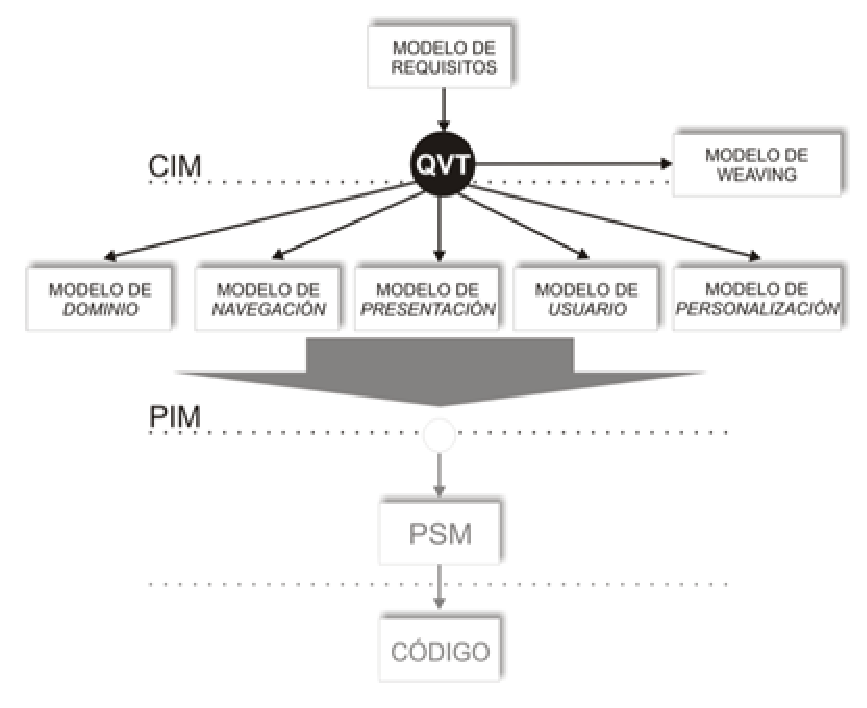
\includegraphics[width=0.8\textwidth]{img/is/approach}
\end{center}
\caption{Overview of our approach} \label{a2:fig:approach}
\end{figure}

The motivation of our work is to provide designers with a set of
transformations in order to ensure summarizability in rich
conceptual models. In this way, designers will be able to implement
a highly expressive conceptual model for any data analysis tool,
without worrying about the kind of complex hierarchies that the tool
supports. The semantic gap between conceptual multidimensional
models and their implementation in a database platform is then
bridged, since an intermediate normalized model is used to provide a
high level of expressiveness in describing multidimensional
structures for real-world situations, while summarizability
conditions are ensured. From this normalized multidimensional model,
an implementation that satisfies summarizability can be easily
deployed in any database platform and can be accurately queried by
any data analysis tool.

The remainder of this paper is structured as follows. We provide
necessary background about MDA, QVT, our UML profile for MD
modeling, and summarizability in the next Section.  In
Sec.~\ref{a2:sec:hierarchies} we then present our viewpoint
concerning the modeling of dimension hierarchies. Afterwards, in
Sec.~\ref{a2:sec:pim}, we describe the definition of different kinds
of dimension hierarchies at the conceptual level, followed by our
normalization process to avoid summarizability problems, which is
implemented on top of the \emph{Eclipse} development platform, in
Sec.~\ref{sec:normalizing}.  We put related work into perspective in
Sec.~\ref{a2:sec:related}.  Finally, we conclude in
Sec.~\ref{a2:sec:conclusions} and sketch potential for future work.
Furthermore, we provide practical examples throughout the paper to
clarify each theoretical concept of our approach.


\section{Background}
\label{a2:sec:background}

\subsection{MDA and QVT} \label{a2:sec:mda} Model Driven Architecture
(MDA) is an Object Management Group (OMG) standard~\cite{OMG/MDA}
that addresses the complete life cycle of designing, deploying,
integrating, and managing applications by using models in software
development. MDA separates the specification of system functionality
from the implementation of that functionality on a specific
technology platform by means of defining several viewpoints on a
system. A viewpoint on a system is a technique for abstracting away
details in order to focus on particular concerns within that system
and to establish a simplified model. MDA defines the following
viewpoints: computation independent, platform independent, and
platform specific. Therefore, MDA encourages specifying a Platform
Independent Model (PIM) which contains no information specific to
the platform or the technology that is used to realize it. This PIM
can be transformed into a Platform Specific Model (PSM) in order to
include information about a specific technology. Afterwards, each
PSM is transformed into code to obtain the final implementation. On
top of these models, MDA also presents a Computation Independent
Model (CIM) to specify user requirements.

These MDA models can be developed using any modeling language, but
typically MOF-compliant languages (such as UML) are used since they
are standardized general purpose modeling languages, which also can
be extended to define specialized languages for certain domains
(i.e., via metamodel extensibility or profiles).

One of the most crucial issue in MDA is the definition of
transformations between models in a formal
way~\cite{OMG/MDA,book/Kleppe/MDA}. These formal transformations
must allow to automatically derive models assuring semantic
correctness~\cite{czarnecki03modeltransformation,DBLP:conf/gg/GerberLRSW02}.
Furthermore, they must be easily readable, understandable,
adaptable, and
maintainable~\cite{DBLP:journals/software/SendallK03}. To this aim,
OMG proposes the MOF 2.0 Query/View/Transformation (QVT)
language~\cite{OMG/QVT}, a standard approach for defining formal
relations between MOF-compliant models.

QVT consists of two parts: declarative and imperative. The
declarative part provides mechanisms to define relations that must
hold between the model elements of a set of candidate models (source
and target models). A set of these relations (or transformation
rules) defines a transformation between models. The declarative part
of QVT can be split into two layers according to the level of
abstraction: the relational layer that provides graphical and
textual notation for a declarative specification of relations, and
the core layer that provides a simpler, but verbose, way of defining
relations. The imperative part defines operational mappings that
extend the declarative part with imperative implementations when it
is difficult to provide a purely declarative specification of a
relation.

In this paper, we focus on the relational layer of QVT. This layer
supports the specification of relationships that must hold between
MOF models by means of a relations language. A QVT relation (see
Fig.~\ref{a2:qvt_example}) is defined by the following elements:
\begin{itemize}
\item \textbf{Two or more domains}: Each domain is a distinguished set of
  elements of a candidate model (source or target model). This set of elements
  (denoted by a \verb"<<domain>>" label, see Fig.~\ref{a2:qvt_example}) must be
  matched in that model by means of patterns. A domain pattern can be
  considered as a template for elements, their properties and their
  associations that must be located, modified, or created in a candidate model
  in order to satisfy the relation. A relation between domains can be marked
  as check-only (labeled as C) or as enforced (labeled as E). When a relation
  is executed in the direction of a check-only domain, it is only checked if
  there exists a valid match in the model that satisfies the relationship
  (without modifying any model if the domains do not match); whereas for a
  domain that is enforced, when the domains do not match, model elements are
  created, deleted, or modified in the target model in order to satisfy the
  relationship. Moreover, for each domain the name of its underlying metamodel
  is specified (labels M1 and M2 in Fig.~\ref{a2:qvt_example}).
\item \textbf{When clause}: This clause specifies the condition under which
  the relation needs to hold (i.e., it forms a precondition). This clause may
  contain arbitrary OCL (Object Constraint Language)~\cite{OMG/OCL}
  expressions in addition to the relation invocation expressions (see
  Fig.~\ref{a2:qvt_example}).
\item \textbf{Where clause}: This clause specifies the condition that must be
  satisfied by all model elements participating in the relation (i.e., it
  forms a postcondition). This clause may also contain OCL expressions or
  relation invocation expressions.
\end{itemize}

\begin{figure}
\begin{center}
\includegraphics[scale=.40]{img/is/qvt_example}
\end{center}
\caption{Example of a QVT relation} \label{a2:qvt_example}
\end{figure}

Defining relations by using the QVT language has the following
advantages:
\begin{enumerate}
\item QVT is a standard language.
\item Relations are formally specified, and transformation engines (e.g.,
  Borland Together Architect~\cite{BORLAND}, SmartQVT~\cite{SMARTQVT},
  mediniQVT~\cite{MEDINI}, or ATL~\cite{ATL}) can execute them automatically.
\item Relations can be easily integrated within an MDA approach.
\end{enumerate}


\subsection{UML Profile for Conceptual MD Modeling}
\label{a2:sec:profile}

Our UML profile for conceptual MD modeling is presented
in~\cite{DBLP:journals/dke/Lujan-MoraTS06}. This profile contains
the necessary stereotypes in order to elegantly represent main MD
properties at the conceptual level. Specifically, the structural
properties of MD modeling are represented by means of a UML class
diagram in which the information is clearly organized into facts and
dimensions. These facts and dimensions are represented by
\textit{Fact} (\includegraphics[height=3mm]{img/icons/fact.png}) and
\textit{Dimension}
(\includegraphics[height=3mm]{img/icons/dimension.png}) classes
respectively. \textit{Fact} classes are defined as composite classes
in shared aggregation relationships of $n$ \textit{Dimension}
classes.

A fact is composed of measures or fact attributes. These are
represented as attributes with the \textit{FactAttribute} stereotype
(\includegraphics[height=2mm]{img/icons/fa.png}). With respect to
dimensions, each level of a hierarchy is specified by a
\textit{Base} class. Every \textit{Base} class
(\includegraphics[height=3mm]{img/icons/base.png}) can contain
several dimension attributes (\textit{DimensionAttribute}
stereotype, \includegraphics[height=2mm]{img/icons/da.png}), one OID
attribute (\textit{OID} stereotype,
\includegraphics[height=2mm]{img/icons/oid.png}),
and must also contain a descriptor attribute (\textit{Descriptor}
stereotype,
\includegraphics[height=2mm]{img/icons/des.png}).
An association (represented by the stereotype \textit{Rolls-UpTo},
\includegraphics[height=3mm]{img/icons/roll.png}) between
\textit{Base} classes specifies the relationship between two levels
of a classification hierarchy.
% The only prerequisite is that these \textit{Base} classes must define a
% \textbf{connected} Directed Acyclic Graph (DAG) rooted in the
% \textit{Dimension} class (this constraint is defined in the \textit{Dimension}
% stereotype).
A \textit{Dimension} class is associated with a unique \textit{Base}
class called \emph{defining dimension level}.
% We don't need the notion of "aggregation path", do we?
%
% An aggregation path is a subsequence of
% \textit{Base} classes, which starts in this defining level (lower
% level of detail) and ends in an implicit level (not graphically
% represented) that represents all the dimension levels.

We use roles to represent the way the two \textit{Base} classes see
each other in a \textit{Rolls-UpTo} association: role \textit{r}
represents the direction in which the hierarchy rolls-up (i.e.,
aggregation), whereas role \textit{d} represents the direction in
which the hierarchy drills-down (i.e., disaggregation).
% Moreover, we use roles to detect and avoid cycles in a classification
% hierarchy, and therefore, help us to achieve the DAG condition.
On the other hand, the multiplicities in these \textit{Rolls-UpTo}
associations allow us to define how the elements within a level are
related with other elements, thus modeling different kinds of
dimension hierarchies.

UML generalization relationships between \textit{Base} classes can
be used to represent optional dimension levels within a hierarchy.
Indeed, when there exist properties (relationships between dimension
levels or dimension attributes) that are only valid for a subset of
elements within a hierarchy level, sparse data cubes as well as
inconsistent queries can arise, which can be avoided by the proper
use of generalization~\cite{DBLP:journals/is/LechtenborgerV03}.

Besides, our approach also allows the definition of degenerate
dimensions~\cite{book/Kimball/DW}, thereby representing other fact
features in addition to the measures for analysis. These degenerate
dimensions are represented as stereotyped attributes of the
\textit{Fact} class (\textit{DegenerateDimension} stereotype,
\includegraphics[height=2mm]{img/icons/dd.png}).

%The definition of analysis
%criteria~\cite{DBLP:journals/dke/MalinowskiZ06} is supported in two
%ways: (i) The same dimension can be related to the same fact with
%different meanings through different associations with different
%names, and (ii) several hierarchies can support different analysis
%criteria, which is supported by naming the corresponding
%\textit{RollsUp-To} associations.

Finally, our profile is formally defined and uses OCL~\cite{OMG/OCL}
for expressing well-formed rules of the newly defined elements,
thereby avoiding their arbitrary use. We refer the reader
to~\cite{DBLP:journals/dke/Lujan-MoraTS06} for a further explanation
of this profile and its corresponding OCL constraints.

\subsection{Summarizability}
\label{a2:sec:summarizability} The notion of \emph{summarizability}
was introduced by Rafanelli and
Shoshani~\cite{DBLP:conf/ssdbm/RafanelliS90} in the context of
statistical databases, where it refers to the correct computation of
aggregate values with a coarser level of detail from aggregate
values with a finer level of detail. Although this seminal work on
summarizability is framed within the context of statistical
databases, it is considered as a cornerstone in MD modeling, because
the authors lay the foundations for detecting and avoiding
summarizability problems in an MD space.

Summarizability as defined by Rafanelli and
Sho\-sha\-ni~\cite{DBLP:conf/ssdbm/RafanelliS90} can be translated
as follows into the language of our UML profile for MD
modeling~\cite{DBLP:journals/dke/Lujan-MoraTS06} presented in the
previous section: Consider a Rolls-UpTo association between two
dimension levels (\textit{Base} classes), say the coarser level
$l_r$ and the finer level $l_d$, and aggregate values for $l_d$.
This association is \emph{summarizable} if ``using'' this
association ``yields the correct summary values'' for $l_r$.
Moreover, Rafanelli and Shoshani observe that many-to-one
associations satisfy summarizability while many-to-many associations
violate summarizability.

In the spirit of \cite{DBLP:conf/ssdbm/RafanelliS90}, Lenz and
Shoshani~\cite{DBLP:conf/ssdbm/LenzS97} argue that summarizability
is of most importance for queries concerning multidimensional data,
since violations of this property may lead to erroneous conclusions
and decisions when data is being analyzed. Correctness of
aggregation results cannot be then guaranteed if summarizability is
not ensured. Therefore, the authors propose three necessary
conditions for summarizability that every dimension hierarchy must
fulfill (disjointness, completeness, and type compatibility).
Although~\cite{DBLP:conf/ssdbm/LenzS97} does not deal with
conceptual modeling of dimension hierarchies, these conditions can
be easily extrapolated to any modeling approach, since they are
somehow related to the relationships between two levels of a
dimension hierarchy, in the following way:

\begin{enumerate}
\item \emph{Disjointness}. This condition checks that a set of instances of one
  hierarchy level can be divided into disjoint subsets when the data is
  disaggregated along the hierarchy. Viewed differently, an instance
  of the finer level can be related to at most one instance of the coarser
  level. For our UML profile for MD modeling, an instance of a
  \textit{Base} class $l_d$ in the role \emph{d} can be related via a
  \textit{Rolls-UpTo} association to at most one instance of the \textit{Base}
  class $l_r$ in the role \emph{r}, in other words the maximum multiplicity in
  the role \emph{r} must be 1.
  For example, in the scenario of Fig.~\ref{a2:fig:sample} the association
  between \textit{Day} and \textit{Week} is disjoint.  In contrast, if
  aggregate sales per \textit{Week} ($=l_d$) are given, then there is no way to
  correctly compute aggregate sales per \textit{Month} ($=l_r$) using the
  many-to-many association between \textit{Week} and \textit{Month} as it is
  unknown how the sales of weeks that partially lie in two months need to be
  divided.

\item \emph{Completeness}. This condition tests that the aggregation of instances at
  one hierarchy level is complete in two ways: (i) all instances at one level
  of the hierarchy exist (no missing elements) and (ii) all instances of one
  level must be related to, at least, one instance of every associated level
  (no unassigned elements). Translated into our MD profile, a \emph{Rolls-UpTo}
  association between \textit{Base} classes in a hierarchy is complete if
  the minimum multiplicity in the role \emph{r} is 1 and the minimum multiplicity in
  the role \emph{d} is 1 as well.  For example, in the scenario of
  Fig.~\ref{a2:fig:sample} the association between \textit{Day} and
  \textit{Week} is complete (every date falls into a week and every week
  consists of at least one day, in fact, of seven days).  In contrast, as the
  association between \textit{Region} and \textit{Country} has multiplicity
  $0$ in the role \emph{d}, the association is incomplete, and the aggregate
  factual values at \textit{Region} cannot be used to compute the ones at
  \textit{Country} (the correct values at \textit{Country} will include
  additional numbers for countries without regions).

\item \emph{Type compatibility}. This condition checks that the statistical function
  associated with the measure is summarizable according to the type of the
  measure (stock, flow and value-per-unit) and the type of the related
  dimensions (temporal, non-temporal). We must check jointly all the
  components of the summarization operation (measure, dimensions and
  statistical function). For the special case where aggregate functions are
  restricted to the \emph{sum} operator, the term \emph{additivity} (instead
  of summarizability) is used frequently.  An in-depth analysis of additivity
  and a taxonomy for reasons why additivity may not hold is presented by
  Horner and Song~\cite{DBLP:conf/er/HornerS05}.  We note that Horner and Song
  distinguish \emph{schema problems}, which are our focus in this paper, from
  \emph{data problems} (e.g., inconsistencies and imprecision) and
  \emph{computational problems} (e.g., type compatibility in the sense of
\cite{DBLP:conf/ssdbm/LenzS97}).
\end{enumerate}

As a side remark we note that in the related literature, two kinds
of completeness are
identified~\cite{DBLP:conf/ssdbm/LenzS97,DBLP:books/idea/mddb2003/PourabbasR03}.
First, some instances may simply be missing in the database (e.g., a
customer may not be recorded in the data warehouse), which is called
incompleteness of type ``omitted'' in~\cite{DBLP:conf/er/HornerS05}.
Second, some instance at a lower level may not be assigned to an
instance of a higher level, which is called ``orphaned''
in~\cite{DBLP:conf/er/HornerS05} and is subsumed by the notion of
completeness given above. We argue that the problem of ``omitted''
instances is a general problem of data quality, which is unrelated
to the design of conceptual or logical models.  Hence, we do not
consider incompleteness of type ``omitted'' any further in this
paper.


\section{Model-driven Design of Dimension Hierarchies}
\label{a2:sec:hierarchies} DW development starts with the definition
of a conceptual MD model whose primary focus is the adequate
description of a given real-world DW scenario without limitations
imposed by technological restrictions.  In particular, non-standard
relationships between dimension levels (e.g., many-to-many or
incomplete relationships, which lead to summarizability problems as
we have seen above) do occur in practice and should be easily
modeled at the conceptual level.  Then, summarizability should be
checked and enforced in a later phase, when the conceptual MD model
is transformed into a logical one as a basis of its implementation
in a specific tool.

However, this transformation is not a trivial task, since both
models are designed with different goals: While a conceptual MD
model should represent the real world in a way that is easy to
understand and that supports discussions with end users, a logical
MD model must support the implementation in a chosen target
technology in such a way that data can be accurately analyzed. To
bridge this semantic gap, we propose to derive an intermediate
model, which should still be expressed at the conceptual level (to
avoid limitations imposed by particular target models) but where MD
structures that violate summarizability conditions are replaced with
summarizable alternatives (which are typically more precise as we
will see below).

To this end, we use MDA (see Sec.~\ref{a2:sec:mda}) to take
advantage of the separation of concerns provided by different models
at different levels of abstraction and to define a normalization
process to transform the designed conceptual MD model into a
constrained conceptual model, which is restricted to those MD
structures that do not violate summarizability, and then into the
logical model. Specifically, we use MDA to specify three kinds of
models with special characteristics and the transformations between
them (see Fig.~\ref{a2:fig:approach}):

\begin{itemize}
\item The \emph{PIM} is a conceptual MD model in which every complex dimension
  hierarchy is modeled as it occurs in the real world, without any
  restrictions regarding summarizability. It must be designed by using a rich
  modeling approach in order to ease the task of the designers to model
  every possible scenario.
\item The \emph{Normalized PIM} is a restricted conceptual MD model. This model
  represents the same scenario as the PIM, but it is restricted in terms of
  the allowed modeling elements, which avoids summarizability problems.
  Moreover, the transformation into a normalized PIM also requires to model
  certain scenarios more precisely, which allows us to resolve
  ambiguities of the original model.
\item The \emph{PSM} represents the MD model at the logical level, i.e., it is
  tailored to one specific technology and serves as basis of the implementation.
\end{itemize}

Our process starts from modeling the PIM.  Then, a normalization
process is carried out in order to obtain a normalized PIM that
ensures summarizability while accurately capturing the
expressiveness of the demanded real-world situation offered by the
PIM. The output of such a process is a conceptual model constrained
to those elements and relationships that do not violate
summarizability (see Fig.~\ref{a2:fig:approach}). From this
normalized PIM, a PSM which ensures consistent results in specific
data analysis tools can be obtained. This process is based on a set
of QVT transformations which allow us to move from the PIM to the
PSM via the normalized PIM.  It is worth pointing out that, in this
paper, we focus on describing the normalization process, as in our
previous works we have addressed the PIM-PSM
transformation~\cite{DBLP:conf/dawak/MazonPT06,journals/dss/Mazon2008}.

We note that this two-step process is advantageous for the following
reasons: First, a manual design of the normalized PIM by the
designer (which would save the first transformation step of our
approach) is tedious and difficult because normalized schemata are
usually more complex and verbose than equivalent ones based on the
full expressiveness of the conceptual model (as ``small''
semantically rich constructs in the PIM may have to be mapped to
multiple concepts in the normalized PIM). Second, one may wonder
whether a single transformation step may be sufficient to obtain the
PSM directly from the PIM.  While such a direct transformation is
possible in theory we argue that our two-step approach is beneficial
in practice: As we first transform some semantically rich constructs
of the PIM at the conceptual level to obtain the normalized PIM, the
subsequent transformations towards the logical level are simplified.
In particular, the design of transformations for different
technologies can be performed with smaller efforts.  Indeed, as we
assure summarizability at the conceptual level in a
technology-independent fashion, transformations targeting new tools
are easier to design, thus obtaining all the advantages of a
model-driven approach.

\section{Designing Dimension Hierarchies in a PIM}
\label{a2:sec:pim} As we have explained in Sec.~\ref{a2:sec:mda}, a
PIM is a view of a system from the platform independent
viewpoint~\cite{OMG/MDA}.  For the purposes of this paper, such a
PIM represents the main properties of an MD scenario at the
conceptual level, and we use our UML
profile~\cite{DBLP:journals/dke/Lujan-MoraTS06} sketched in
Sec.~\ref{a2:sec:profile} to specify such PIMs.  As shown in
Sec.~\ref{a2:sec:summarizability}, in case of complex dimension
hierarchies the conditions guaranteeing
summarizability~\cite{DBLP:conf/ssdbm/LenzS97} may not hold.
Nevertheless, as such complex hierarchies do occur in real-world
scenarios, they need to be supported by rich conceptual MD models to
satisfy the information needs of decision makers, and our primary
goal in this section is to systematically analyze summarizability
issues for all kinds of relationships among dimension levels that
designers may want to use.

We emphasize that although several authors stress the importance of
support for ``irregular'' hierarchies, e.g,
\cite{DBLP:journals/tods/HurtadoGM05,DBLP:journals/vldb/JensenKPT04,DBLP:journals/dke/MalinowskiZ06,MalZim2008:book,MansmannIJDWDM07},
our proposal considers individual relationships between \emph{pairs}
of hierarchy levels (i.e. \textit{Base} classes) instead of
\emph{entire} hierarchies, which ease the task of designers thanks
to the following advantages:

\begin{enumerate}
\item We explicitly list all elementary modeling constructs.  Hence, in the
  first place it is clear which modeling constructs are available.
  Consequently, complex hierarchies can be designed incrementally by focusing
  on one individual relationship between levels at a time.

\item We are in the position to analyze the summarizability properties of all
  constructs, and we are able to distinguish problematic ones from safe ones.

\item The summarizability issues for each problematic construct can be
  resolved individually.

\item Our transformation from PIM to normalized PIM is defined modularly by a
  composition of the individual transformations for the problematic constructs.
\end{enumerate}

Based on the features of our UML profile we next present a
systematic and complete, yet simple characterization of \emph{all}
possible kinds of relationships among pairs of \textit{Base} classes
(i.e., hierarchy levels).  To this end, we observe that a
``relationship'' in our UML profile may either be a
\textit{Rolls-UpTo} association or a generalization. In the
following subsection we first concentrate on the impact of
multiplicities attached to association ends and address
generalization afterwards.

\subsection{Impact of Multiplicities}
In our MD profile, \textit{Rolls-UpTo} associations between
\textit{Base} classes are annotated with multiplicities. As pointed
out in Sec.~\ref{a2:sec:summarizability}, many-to-one associations
are at the core of every MD model, and they do not pose any
summarizability problems. Other multiplicities, however, are known
to form ``irregular'' hierarchies with summarizability problems. In
view of that observation in
Tab.~\ref{a2:tab:multiplicity-classification} we present a complete
characterization of \textit{Rolls-UpTo} associations based on the
minimum and maximum multiplicities used in the roles \emph{d} and
\emph{r}. In that table ``regular'' and ``unusual'' denote
association types without summarizability problems, the latter being
rarely used, whereas the remaining entries form a selection of terms
used in the literature for a particular irregularity; the ones used
in this paper are \emph{emphasized} and explained in the following.
In particular, we propose the novel terms ``drill-down incomplete''
and ``roll-up incomplete'', which convey a figurative meaning that
we hope to be easy to remember.  We next describe all cases in
detail.

\begin{table}
  %\tiny
  \centering
  \caption{Classification of \textit{Rolls-UpTo} associations between \textit{Base} classes}
  \label{a2:tab:multiplicity-classification}
    \begin{tabular}{|c||c|c|c|c|}
         \hline
       & \multicolumn{2}{|c|}{Minimum Multiplicity} & \multicolumn{2}{|c|}{Maximum Multiplicity} \\\hline
       & 0 & 1 & 1 & * \\\hline
      Role \emph{d} & \emph{drill-down incomplete}, asymmetric, non-onto, unbalanced & regular & unusual & regular \\
      Role \emph{r} & \emph{roll-up incomplete}, incomplete, non-covering, ragged, orphaned & regular &  regular & \emph{non-strict} \\\hline
    \end{tabular}
\end{table}

%\begin{table}
%  \centering
%  \caption{Classification of associations between dimension levels}
%  \label{tab:cardinality-classification}
%  \begin{tabular}{cc}
%    \begin{tabular}{|c||c|c|}
%       \multicolumn{3}{c}{Minimum Multiplicity}\\\hline
%      & 0 & 1 \\\hline
%      Role D & \emph{asymmetric}, non-onto, unbalanced & regular \\
%      Role R & \emph{incomplete}, non-covering, ragged & regular \\\hline
%    \end{tabular}
%    &
%    \begin{tabular}{|c||c|c|}
%       \multicolumn{3}{c}{Maximum Multiplicity} \\\hline
%      & 1 & * \\\hline
%      Role D & regular (yet unusual) & regular \\
%      Role R & regular & \emph{non-strict}\\\hline
%    \end{tabular}
%  \end{tabular}
%\end{table}

\subsubsection{Regular Situations}
We note that summarizability of the ``regular'' entries follows from
the necessary conditions \emph{disjointness} and \emph{completeness}
for summarizability stated in \cite{DBLP:conf/ssdbm/LenzS97}.
Indeed, disjointness implies that the maximum multiplicity at role
\emph{r} is $1$ while completeness implies that the minimum
multiplicities at both roles are $1$.  Furthermore, the maximum
multiplicity at role \emph{d} is usually $*$, but this multiplicity
may be $1$, which is an unusual situation for OLAP scenarios but
which does not contradict the necessary conditions of
\cite{DBLP:conf/ssdbm/LenzS97}. Examples of regular situations can
be observed in Fig.~\ref{a2:fig:sample} between \emph{Product} and
\emph{Brand} (one product belongs to only one brand, and a brand can
have several products) or between \emph{Month} and \emph{Year} (one
month belongs to one year, while a year is composed of several
months).

\subsubsection{Drill-down Completeness}
A \textit{Rolls-UpTo} association involving a pair of \textit{Base}
classes is \emph{drill-down complete} if for every element $e$ of
the coarser \textit{Base} class (i.e., role \emph{r}, such as
\textit{Country} for the association between \textit{City} and
\textit{Country}) there exists an element at the finer \textit{Base}
class (i.e., role \emph{d}, here \textit{City}) which is associated
with element $e$; otherwise, it is called \emph{drill-down
incomplete}.  In other words, a \textit{Rolls-UpTo} association is
drill-down incomplete if the minimum multiplicity at role \emph{d}
is $0$; otherwise, it is drill-down complete. For example, the
association between \textit{Country} and \textit{Region} in
Fig.~\ref{a2:fig:sample} is drill-down incomplete as there are
countries (such as ``Andorra'', ``Monaco'', etc.)  without
associated regions.

As illustrated in Tab.~\ref{a2:tab:DrillDownIncompleteness},
drill-down incompleteness violates summarizability since it may
yield inconsistent totals. We show the sales by region in
Tab.~\ref{a2:tab:DrillDownIncompletenessA}, where the total amount
is $60$. However, if we try to roll-up to country (see
Tab.~\ref{a2:tab:DrillDownIncompletenessB}), we have to be careful
because countries without regions need also to be taken into account
and the total sales change to $70$. Here, the reason of these
inconsistent values is that ``Westfalen'', ``Bayern'' and
``Rheinland'' are german regions, ``Valencia'' and ``Murcia'' are
spanish regions, but ``Andorra'' has no associated regions and,
therefore, its sales are not considered in aggregations by region.


\begin{table}
\centering \caption{Inconsistent totals for sales due to drill-down
incompleteness}
     \label{a2:tab:DrillDownIncompleteness}
\subtable[Sales by region] {
        \label{a2:tab:DrillDownIncompletenessA}
        \begin{tabular}{|c|c|}
        \hline
        Region & Sales \\
        \hline
        \hline
        Westfalen & 10 \\
        Bayern & 5 \\
        Rheinland & 10 \\
        Valencia & 15 \\
        Murcia & 20 \\
        \hline
        Total & 60 \\
        \hline
        \end{tabular}
} \qquad\qquad \subtable[Sales by country] {
     \label{a2:tab:DrillDownIncompletenessB}
        \begin{tabular}{|c|c|}
        \hline
        Country & Sales \\
        \hline
        \hline
        Germany & 25 \\
        Spain & 35 \\
        Andorra & 10 \\
        \hline
        Total & 70 \\
        \hline
        \end{tabular}
}
\end{table}


\subsubsection{Roll-up Completeness}
A \textit{Rolls-UpTo} association involving a pair of \textit{Base}
classes is \emph{roll-up complete} if for every element $e$ of the
finer \textit{Base} class (i.e., role \emph{d}, such as
\textit{Product} for the association between \textit{Product} and
\textit{Brand}) there exists an element at the coarser \textit{Base}
class (i.e., role \emph{r}, here \textit{Brand}) which is associated
with element $e$; otherwise, it is called \emph{roll-up incomplete}.
In other words, a \textit{Rolls-UpTo} association is roll-up
incomplete if the minimum multiplicity at role \emph{r} is $0$;
otherwise, it is roll-up complete. For example, the association
between \textit{Product} and \textit{Category} in
Fig.~\ref{a2:fig:sample} is roll-up incomplete, and faces the
problem of inconsistent totals as shown in
Tab.~\ref{a2:tab:RollUpIncompleteness}, where we assume that
``milk'' and ``beer'' belong to category ``drink'', ``bread'' and
``tuna'' to category ``food'', and ``napkin'' has no category.
Therefore, when factual data is aggregated by product the sales are
$60$ (see Tab.~\ref{a2:tab:RollUpIncompletenessA}). However, special
attention should be paid when data is aggregated by category, since
``napkin'' sales are not taken into account and the total sales
decrease to $40$ (as shown in
Tab.~\ref{a2:tab:RollUpIncompletenessB}).

\begin{table}
\centering \caption{Inconsistent totals for sales due to roll-up
incompleteness}
     \label{a2:tab:RollUpIncompleteness}
\subtable[By product] {
        \label{a2:tab:RollUpIncompletenessA}
        \begin{tabular}{|c|c|}
        \hline
        Product & Sales \\
        \hline
        \hline
        Milk & 10 \\
        Beer & 5 \\
        Bread & 10 \\
        Tuna & 15 \\
        Napkin & 20 \\
        \hline
        Total & 60 \\
        \hline
        \end{tabular}
} \qquad\qquad \subtable[By category] {
     \label{a2:tab:RollUpIncompletenessB}
        \begin{tabular}{|c|c|}
        \hline
        Category & Sales \\
        \hline
        \hline
        Drink & 15 \\
        Food & 25 \\
        \hline
        Total & 40 \\
        \hline
        \end{tabular}
}
\end{table}


\subsubsection{Strictness}
A \textit{Rolls-UpTo} association involving a pair of \textit{Base}
classes is \emph{strict} if for every element $e$ of the finer
\textit{Base} class (i.e., role \emph{d}, such as \textit{Day} for
the association between \textit{Day} and \textit{Week}) there exists
at most one element at the coarser \textit{Base} class (i.e., role
\emph{r}, here \textit{Week}) which is associated with element $e$;
otherwise, it is called \emph{non-strict}.  In other words, a
\textit{Rolls-UpTo} association is non-strict if the maximum
multiplicity at role \emph{r} is $*$; otherwise, it is strict. For
example, the association between \textit{Week} and \textit{Month} in
Fig.~\ref{a2:fig:sample} is non-strict, and requires special care to
avoid the well-known double counting problem, which is illustrated
in Tab.~\ref{a2:tab:NonStrictness}: As week ``5-2008'' partially
belongs to ``January'' as well as ``February'' (see
Tab.~\ref{a2:tab:NonStrictnessA}), the sales for week ``5-2008''
should not be counted twice (as is done in
Tab.~\ref{a2:tab:NonStrictnessB}) but should be divided
appropriately among both months.

\begin{table}
\centering \caption{Double counting problem for sales due to
non-strictness}
     \label{a2:tab:NonStrictness}
\subtable[Sales by week] {
        \label{a2:tab:NonStrictnessA}
        \begin{tabular}{|c|c|}
        \hline
        Week & Sales \\
        \hline
        \hline
        4-2008 & 10 \\
        5-2008 & 20 \\
        6-2008 & 10 \\
        7-2008 & 10 \\
        8-2008 & 10 \\
        9-2008 & 10 \\
        \hline
        Total & 70 \\
        \hline
        \end{tabular}
} \qquad\qquad \subtable[Sales by month] {
     \label{a2:tab:NonStrictnessB}
        \begin{tabular}{|c|c|}
        \hline
        Month & Sales \\
        \hline
        \hline
        Jan-2008 & 30 \\
        Feb-2008 & 60 \\
        \hline
        Total & 90 \\
        \hline
        \end{tabular}}
\end{table}


\subsection{Generalization}
\label{a2:sec:generalization} As observed by Lehner et
al.~\cite{DBLP:conf/ssdbm/LehnerAW98}, dimension levels in MD models
may exhibit heterogeneity in the sense that certain properties may
only be applicable to a subset of elements. E.g., for the dimension
level \textit{Customer} in the scenario shown in
Fig.~\ref{a2:fig:sample}, some customers can be categorized by their
\textit{Gender} (if they are human beings) and others by
\textit{Branch} (if they are companies).  If those properties are
modeled as \textit{Base} classes, which are reachable from the
\textit{Base} class \textit{Customer} via \textit{Rolls-UpTo}
associations, then those associations will necessarily suffer from
roll-up incompleteness and the inherent summarizability problems
(see Fig.~\ref{heterogeneity1}).
%Falta poner aqu� el CustomerType
Moreover, as explained in~\cite{DBLP:conf/ssdbm/LehnerAW98}, sparse
data cubes may result, and users may pose inconsistent queries
(``show sales by gender and branch usage''). From an object-oriented
perspective such heterogeneity indicates the existence of
sub-classes where the individual properties are either applicable
(as attributes) or not. In fact, this perspective guides the
definition of the third multidimensional normal
of~\cite{DBLP:journals/is/LechtenborgerV03}, where context
dependencies explain the applicability of dimension levels;
moreover, these dependencies can be used to construct class
hierarchies that contain the applicable attributes, which avoids
roll-up incompleteness and associated summarizability problems.  It
is instructive to note, however,
that~\cite{DBLP:journals/is/LechtenborgerV03} does \emph{not} allow
generalizations as modeling constructs. Moreover, although several
MD design proposals are based on object-oriented modeling and, in
particular, the
UML~\cite{DBLP:journals/is/AbelloSS06,DBLP:journals/dke/Lujan-MoraTS06,DBLP:journals/dss/PratAC06}
none of them explicitly suggests the use of generalization to avoid
roll-up incompleteness. Hence, we next explain in detail how
generalization may be exploited in order to avoid summarizability
problems when data is being analyzed.

\begin{figure}
\subfigure[Use of roll-up incompleteness]{
\includegraphics[width=0.5\textwidth]{img/is/heterog1.png}
\label{heterogeneity1}} \subfigure[Use of generalization]{
\includegraphics[width=0.5\textwidth]{img/is/heterog2.png}
\label{heterogeneity2}} \caption{Modeling heterogeneity}
\end{figure}

In particular, generalization relationships for dimension levels
embody an attractive alternative for roll-up incomplete
associations. Indeed, with generalization, new analysis potential is
unleashed as indicated in~\cite{DBLP:journals/is/LechtenborgerV03}:
\begin{enumerate}
\item Traditional roll-up operations may be performed within a certain
  sub-class by using only the applicable levels, which now provides
  context-sensitive summarizability.  E.g., in Fig.~\ref{a2:fig:sample}
  (and also in the excerpt shown in Fig.~\ref{heterogeneity2})
  if an
  analyst switches the context from sales of all individual \textit{Customer}s to
  those related to \textit{Private} customers, it is clear that the sales
  related to \textit{Company} customers will be ignored and it is now safe to
  roll-up to \textit{Gender} without summarizability problems
  as they are applicable to \textit{Private} customers. The more verbose way of modeling heterogeneity shown in
  Fig.~\ref{heterogeneity2} should be contrasted with the traditional
  alternative shown in Fig.~\ref{heterogeneity1}.
\item A novel type of drill-down operation allows to switch from a \textit{Base}
  class to its immediate sub-classes.  E.g., in Fig.~\ref{heterogeneity2}
  aggregate sales for all \textit{Customer}s can be split into sales for
  \textit{Company} and \textit{Private} customers (or in the opposite
  direction via a novel type of roll-up).
\end{enumerate}

Some observations concerning these types of operations are apt. With
respect to case (1) we note that actually two types of data analysis
operations are involved: First, an analyst needs to perform a novel
type of operation, which we call \emph{context switch}. This
operation restricts the members of some dimension level to those of
a sub-class (e.g., from \textit{Customer} to \textit{Private}
above). Interestingly, a context switch operation aims to restrict
the \textit{Base} class instances to a subset, so it remains data at
the same level of detail and it does not present summarizability
problems. Therefore, afterwards, the usual data analysis operations
are applicable, starting from the dimension level of the chosen
sub-class.

With respect to case (2) it is instructive to analyze in what
situations the novel type of data analysis operation, which we call
\emph{sub-class split}, can be applied. It turns out that a
sub-class split from a parent level $l_p$ to sub-classes is
applicable if the current analysis context is determined by $l_p$.
This sub-class split is a type of aggregation operation that changes
the level of detail when data is analyzed, thus poses some
challenges to avoid summarizability problems. In traditional MD
modeling approaches a sub-class split can be simulated by
introducing a new dimension level that captures the immediate
sub-classes. A simulation of this way of proceeding is shown in
Fig.~\ref{heterogeneity1}, where there is a \textit{Rolls-UpTo}
association from the parent \textit{Base} class \textit{Customer}
(role \emph{d}) to the new \textit{Base} class \textit{CustomerType}
(role \emph{r}). The instances of this new \textit{Base} class will
be ``Company'' or ``Private''. It is easy to see that this
association has
\begin{itemize}
\item multiplicity $1..1$ at role \emph{r} if the generalization is complete and
  disjoint,
\item multiplicity $0..1$ at role \emph{r} if the generalization is incomplete
  and disjoint,
\item multiplicity $1..*$ at role \emph{r} if the generalization is complete
  and overlapping, and
\item multiplicity $0..*$ at role \emph{r} if the generalization is incomplete
  and overlapping.
\end{itemize}
Consequently, the novel sub-class split is summarizable for complete
and disjoint generalizations, whereas other cases exhibit the
summarizability issues of roll-up incomplete and/or non-strict
associations seen above.

We briefly recall from~\cite{DBLP:journals/is/LechtenborgerV03} that
generalizations can always be turned into complete and disjoint
ones: Incomplete generalizations can be ``completed'' by introducing
an additional sub-class that contains those instances of the
super-class that are not covered by any existing sub-class.
Overlapping sub-classes can be turned into disjoint ones by
introducing new sub-classes to cover the instances in intersections
of previously overlapping classes.  As such schema transformations
generate sub-classes that may not be desirable for analysis
purposes, we do not propose to enforce completeness and disjointness
at all costs.  Instead, we require that all generalizations are
annotated (via standard UML mechanisms) whether they are complete
and disjoint or not.  Based on these schema annotations, advanced
OLAP tools can then offer the novel sub-class split operation for
complete and disjoint generalizations, while it will not be
available for other generalization types.

In any case, we advocate to keep generalization at the normalized
PIM and to transform generalization relationships into other data
structures at the logical level (PSM level), depending on the
implementation platform. Indeed, several platforms allow the direct
implementation of these structures, e.g., starting with SQL:1999,
the SQL standards support the direct implementation of
generalization. On the other hand, incomplete relationships will be
transformed into generalization in the normalized PIM in order to
obtain a more precise model.


\subsection{Guidelines to Design Dimension Hierarchies}
Users of semantically rich modeling techniques, such as our UML
profile for MD modeling, should be supported by guidelines to ease
the design process and to avoid common pitfalls. In the following we
propose a set of such guidelines concerning the conceptual design of
complex dimension hierarchies.

\subsubsection{Forbidden Multiplicities}
Some combinations of multiplicities simply do not make sense for
\textit{Rolls-UpTo} associations: Since the roles \emph{d} and
\emph{r} indicate the direction in which the data is aggregated
(\emph{r}) or disaggregated (\emph{d}), the maximum multiplicity on
the role \emph{d} must be greater than or equal to the maximum
multiplicity on the role \emph{r}.

\subsubsection{Multiplicities of Fact-Dimension Relationships}
We assume that all fact-dimension relationships are complete, i.e.,
that the multiplicity in the role of the \textit{Dimension} class is
1, which indicates that every fact is always related to all the
dimensions. We note that this is not a severe restriction as other
types of fact-dimension relationships can be transformed into
complete ones via the techniques proposed in~\cite{MLT08}.

% \subsubsection{Special multiplicity for the defining dimension level}
% As commented in Sec.~\ref{a2:sec:profile}, a \textit{Dimension} class is
% associated with a unique \textit{Base} class, called defining
% dimension level. This association should have multiplicity 1 in both
% ends as the defining level determines the granularity of its dimension.

\subsubsection{Explicitly Define Essential Associations between \textit{Base} Classes}
In general, dimension hierarchies represent only immediate
parent-child associations between \textit{Base} classes, while
associations that can be derived are
omitted~\cite{DBLP:books/idea/mddb2003/PourabbasR03}.  E.g., in
Fig.~\ref{a2:fig:sample} as every \textit{Customer} is located in
exactly one \textit{City} and as every \emph{City} is located in
exactly one \textit{Country}, we can infer a (transitive)
many-to-one association between \textit{Customer} and
\textit{Country}, which does not need to be modeled explicitly.

However, as observed in \cite{DBLP:journals/vldb/JensenKPT04}, when
different types of relationships are used some care is necessary to
determine which relationships are redundant and which are actually
essential. In \cite{DBLP:journals/vldb/JensenKPT04} in the context
of geo-data, \emph{partial} containment relationships are
distinguished from \emph{full} ones, where partial containment
relationships roughly correspond to our notion of non-strict
associations.  E.g., if a geographical \textit{Coordinate} lies on a
\textit{Road} then it is fully contained, while a \textit{Road}
typically is only partially contained in a \textit{City} because it
runs through many \textit{Cities}.  In this situation, one needs to
model explicitly that a \textit{Coordinate} is also fully contained
in a \textit{City} because this information \emph{cannot} be derived
via the relationships from \textit{Coordinate} to \textit{Road} to
\textit{City}.

Similarly, in Fig.~\ref{a2:fig:sample} we have a strict association
between \textit{Day} and \textit{Week} followed by a non-strict one
between \textit{Week} and \textit{Month}.  In this situation, we
need to model the \emph{strict} association from \textit{Day} to
\textit{Month} explicitly, as otherwise we could only infer a
non-strict one.  Generally speaking, if no other type of association
between \textit{Base} classes can be inferred, then a many-to-many
relationship can always be assumed, as this is the least restrictive
case.

\subsubsection{Expressing Optionality between \textit{Base} Classes}
Different approaches provide different mechanisms to indicate that
certain \textit{Base} classes may be optional: Early approaches such
as~\cite{DBLP:journals/ijcis/GolfarelliMR98} just allow to use
special schema annotations that indicate optionality, in which case
attributes will sometimes have null values that lead to
summarizability problems.  Other approaches such
as~\cite{DBLP:journals/tods/HurtadoGM05,DBLP:journals/is/LechtenborgerV03,DBLP:journals/dke/MalinowskiZ06}
allow to include multiple alternative paths within a hierarchy.  In
particular,
\cite{DBLP:journals/tods/HurtadoGM05,DBLP:journals/is/LechtenborgerV03}
introduce special kinds of constraints that allow to reason about
summarizability in the presence of optional \textit{Base} classes.

In line with the general analysis concerning optional properties for
conceptual design in~\cite{Bodart01} we argue that multiplicities of
$0$ should be avoided in \emph{understandable} conceptual models
whenever possible.  Instead, we advocate to apply generalization for
conceptual MD modeling as well.  Indeed, as shown in our sample
scenario the sub-classing of \textit{Customers} into
\textit{Private} customers and \textit{Companies} allows to
represent alternative aggregation paths intuitively and cleanly.
More generally, we advocate to model generalization relationships
between \textit{Base} classes to represent optional dimension
properties and hierarchy levels, thus allowing context-sensitive
summarizability in a way that it is easy to understand by designer
and users.  Therefore, more complex mechanisms that could mislead
designers and users are avoided.

However, as designers are currently not familiar with the direct use
of generalization instead of incomplete associations, we encourage
them to mix these two options in the PIM according to their
experience.  Specifically, we advocate to prefer generalization if
sub-classes can be identified \emph{a priori}, and every sub-class
has specific properties.  For example, in Fig.~\ref{a2:fig:sample},
we know beforehand that there are two kinds of customers and that
they have different properties (a private customer has birthdate and
can be aggregated by gender, while a company has a contact person
and can be aggregated by branch).  Otherwise, roll-up incompleteness
may be preferable.  For example, in Fig.~\ref{a2:fig:sample}, we do
not know in advance the quantity of categories for the products
(even worse, new categories may need to be added).  Besides, every
category has the same properties (all have a name and all belong to
a class).  Therefore, this last scenario is modeled by means of
roll-up incompleteness.

Even if MD scenarios appear to require incompleteness at first
sight, which can be modeled easily, further investigation by the
designer may reveal that generalization allows to model the
situation more precisely. Therefore, our normalization process is
useful for obtaining the generalizations which are equivalent to the
incomplete relationships between \textit{Base} classes, thus
supporting designers in choosing between different design
alternatives.


\section{Normalizing Dimension Hierarchies to Ensure Summarizability}
\label{sec:normalizing} A normalization process is carried out in
order to obtain a conceptual MD model that ensures summarizability
while accurately capturing the expressiveness of the demanded
real-world situation. The output of such a process is a normalized
PIM constrained to hierarchies that contain only those elements and
relationships that do not violate summarizability. From this
normalized PIM, an implementation which ensures consistent results
in data analysis tools can be obtained.

\subsection{Normalized PIM} \label{sec:normalizedPIM}
Our normalization process is done at the conceptual level (recall
Fig.~\ref{a2:fig:approach}), by using schema information, in
contrast to consider only data instances for avoiding
summarizability problems (as advocated
in~\cite{DBLP:journals/is/PedersenJD01}), which may be an unsuitable
solution due to the huge size of data sources in DW systems.
Importantly, instance-level solutions require complex preprocessing
tasks (e.g., every time the data warehouse is updated, the
normalization process must be executed) which can result in
performance problems.  Moreover, the instance-level solution
by~\cite{DBLP:journals/is/PedersenJD01} algorithmically ``invents''
new dimension levels and new dimension instances, which may not have
natural counterparts in the real-world, thus resulting in an
artificial solution that complicates the use of a data analysis
tool. Conversely, our schema-level solution applies a normalization
process to check and enforce the right multiplicities in the schema.

Once all dimension hierarchies are modeled in a PIM (according to
the previous section), our goal is to obtain a normalized PIM, which
conforms with the summarizability conditions for MD models (see
Sec.~\ref{a2:sec:summarizability}).  To this end, the normalized PIM
should be restricted to the following set of elements and
relationships that avoid summarizability problems:

\begin{itemize}
    \item \textit{Dimension} classes.
    \item \textit{Fact} classes (including \emph{FactAttribute} and \emph{DegenerateDimension} properties).
    \item \textit{Rolls-UpTo} associations with the multiplicities of
      ``regular'' or ``unusual'' situations (see Sec.~\ref{a2:sec:hierarchies}):
      minimum multiplicity $1$ in role \emph{d} (maximum multiplicity makes no
      difference) and minimum and maximum multiplicity $1$ in
      role \emph{r}.
    \item Generalization between \textit{Base} classes: as explained in
      Sec.~\ref{a2:sec:generalization}, the novel operations context-switch and
      sub-class split, which are based on generalization relationships,
      prevent summarizability problems at the conceptual level.
\end{itemize}


\subsection{PIM to Normalized PIM Transformation}
\label{a2:sec:transformation1} We are now in the position to develop
a set of transformations that replaces each of those
(non-normalized) \emph{Rolls-UpTo} associations that violate
summarizability with different (normalized) ones that preserves the
meaning of the original PIM by using a restricted set of elements.
(In fact, we obtain a more precise representation from which the
original PIM can be reconstructed algorithmically.)

We now present a set of QVT transformations to establish formal and
automatic transformations between the PIM and the normalized PIM.
For the sake of understanding, these transformations are first
defined informally and then described formally according to the
declarative part of QVT (see Sec.~\ref{a2:sec:mda}). Afterwards, we
argue for each transformation that it is sound in the following
sense: If some data can be stored under a given source model then it
must be possible to store that data (possibly transformed) in such a
way under the target model that the original data can be restored
without loss of information.

It is worth noting that our QVT transformations focus on matching in
the PIM those \textit{Rolls-UpTo} associations between \textit{Base}
classes which present summarizability problems (drill-down
incompleteness, roll-up incompleteness or non-strictness), thus
obtaining an equivalent set of elements in the normalized PIM to
avoid them (see Fig.~\ref{a2:fig:normalization}). In particular, we
define a QVT relation for each summarizability problem. Once each of
these QVT relations is applied in the PIM (i.e., input model), a new
model (i.e., output model) is obtained in which only the
summarizability problem under study is normalized.

\begin{figure}
\begin{center}
\includegraphics[width=0.8\textwidth]{img/is/normalization.png}
\end{center}
\caption{Overview of our normalization process}
\label{a2:fig:normalization}
\end{figure}


Note that the developed QVT transformations can be applied modularly
in order to eliminate each time one of the summarizability problems.
This is an important advantage of our approach because we can use
either all or only a subset of the transformations depending on the
summarizability problems we want to eliminate. E.g., if the tool
chosen to implement the DW supports non-strict associations in an
adequate way, then there is no need to eliminate non-strict
associations. Hence, the corresponding QVT transformation can be
omitted easily.


\subsubsection{Eliminating Drill-down Incompleteness}
The transformation that eliminates drill-down incompleteness is
based on one QVT relation that replaces all occurrences of
drill-down incomplete \textit{Rolls-UpTo} associations with
normalized elements. The rationale of this QVT relation is removing
summarizability problems by using generalization constructs, in such
a way that the optional \textit{Base} class (which has multiplicity
$0$ at the role \emph{d}, e.g., \emph{Region} in
Fig.~\ref{a2:fig:sample}) should be associated with a sub-class in a
generalization between \textit{Base} classes.

The corresponding QVT relation (named as
\emph{drillDownIncompleteBases}) is shown in
Fig.~\ref{a2:fig:drilldownincomplete} where drill-down incomplete
\textit{Rolls-UpTo} associations between \textit{Base} classes are
detected in the source model by checking if there is a multiplicity
$0$ in the role \emph{d} of the association, say the association $s$
between $b_1$ in the role \emph{d} (e.g., \emph{Region} in
Fig.~\ref{a2:fig:sample}) and $b_2$ in the role \emph{r} (e.g.,
\emph{Country} in Fig.~\ref{a2:fig:sample}). If this situation is
matched in the source model, then the following set of elements are
created in the target model: Two new \textit{Base} classes $b_1p$
and $b_2p$ that correspond to the source \emph{Base} classes $b_1$
and $b_2$, respectively. In addition, two new \textit{Base} classes
are created: $b_3$ as sub-class of $b_2p$ via a new generalization
relationship $g_1$ and $b_4$ as sub-class of $b_2p$ via a new
generalization relationship $g_2$. Moreover, a new drill-down
complete \textit{Rolls-UpTo} association $r$ with $b_1p$ in role
\emph{d} and $b_3$ in role \emph{r} replaces the previous drill-down
incomplete association.

\begin{figure}
     \centering
     \includegraphics[width=\textwidth]{img/is/drilldownincomplete.png}
     \caption{QVT relation to eliminate drill-down incompleteness}
     \label{a2:fig:drilldownincomplete}
\end{figure}

After the execution of the \emph{drillDownIncompleteBases} relation,
an excerpt of the target model related to the \emph{Customer}
dimension is shown in Fig.~\ref{a2:fig:outdrilldowninc}.  Here, two
new \textit{Base} classes \emph{CountryWRegion} and
\emph{CountryWORegion} are created, which are children in a
generalization relationship of the \emph{Country} \textit{Base}
class.  Moreover, the previously drill-down complete relation
between \emph{Region} and \emph{Country} is replaced by a complete
one between \emph{Region} and \emph{CountryWRegion}.  It is worth
noting that those parts of the source model that do not suffer from
drill-down incompleteness are copied directly to the target model.

\begin{figure}
     \centering
     \includegraphics[width=0.7\textwidth]{img/is/outdrilldowninc.png}
     \caption{Excerpt of the target model for the \emph{Customer} dimension}
     \label{a2:fig:outdrilldowninc}
\end{figure}

With respect to the soundness of the \emph{drillDownIncompleteBases}
relation, we focus on the drill-down incomplete association of the
source model, say association $s$ between $b_1$ in the role \emph{d}
and $b_2$ in the role \emph{r}, which is represented differently in
the target model.  First, $b_1$ and $b_2$ are still present in the
target model (as $b_1p$ and $b_2p$, respectively). Moreover, if an
instance of $b_2$ is not related to any instance of $b_1$ (which
exemplifies the incompleteness of the association) then this
instance is simultaneously stored as an instance of $b_2p$ and $b_4$
under the target model. If, however, an instance $i_2$ of $b_2$ is
related to some instance $i_1$ of $b_1$ in the source model, then in
the target model $i_2$ will be an instance of $b_2p$ \emph{and}
simultaneously an instance of $b_2p$'s sub-class $b_3$.  Now, this
sub-class $b_3$ has a drill-down complete association with $b_1p$,
which allows to retrieve the associated instance $i_1$ in the target
model.  Hence, the information that can be represented under the
source model can also be represented under the target model.


\subsubsection{Eliminating Roll-up Incompleteness}

To eliminate roll-up incompleteness, the transformation is based on
one QVT relation that replaces all occurrences of roll-up incomplete
\textit{Rolls-UpTo} associations in the source model with
generalization constructs. In this case, the optional \textit{Base}
class (which has multiplicity $0$ at the role \emph{r}) should be
associated with a suitable sub-class in a generalization between
\textit{Base} classes: one to reflect instances with the optional
property and the other one to reflect instances without that
property.

The corresponding QVT relation (\emph{rollUpIncompleteBases}) is
shown in Fig.~\ref{a2:fig:rollupincomplete}. It checks roll-up
incompleteness in the \textit{Rolls-UpTo} association between
\textit{Base} classes in the source model. Specifically, if a $0$
multiplicity is detected in the role \emph{r} of a
\textit{Rolls-UpTo} association $s$ between two \textit{Base}
classes $b_1$ (e.g., \emph{Product} in Fig.~\ref{a2:fig:sample}) and
$b_2$ (e.g., \emph{Category} in Fig.~\ref{a2:fig:sample}), then the
relation enforces the creation of new elements in the target model
as follows: Two new \textit{Base} classes $b_1p$ and $b_2p$ that
correspond to the source \emph{Base} classes $b_1$ and $b_2$,
respectively. In addition, two new \textit{Base} sub-classes of
$b_1p$, namely $b_3$ and $b_4$, are created via new generalization
relationships $g_1$ and $g_2$. Here, $b_3$ reflects the instances of
its super-class $b_1p$ that are associated with some instance of the
optional \textit{Base} class $b_2p$, and $b_4$ reflects the
remaining instances of $b_1p$. Furthermore, the roll-up incomplete
association $s$ between $b_1$ and $b_2$ is replaced with a roll-up
complete association $r$ between $b_3$ and $b_2p$.

\begin{figure}
     \centering
     \includegraphics[width=\textwidth]{img/is/rollupincomplete.png}
     \caption{QVT relation to eliminate roll up incompleteness}
     \label{a2:fig:rollupincomplete}
\end{figure}

After the execution of the \emph{rollUpIncompleteBases} relation, an
excerpt of the target model related to the \emph{Product} dimension
is shown in Fig.~\ref{a2:fig:outrollupinc}. Here, two new
\textit{Base} classes, \emph{ProductWCategory} and
\emph{ProductWOCategory}, are created to reflect those products that
belong to a category or not, respectively. Again, those parts of the
source model that do not present roll-up incompleteness problems are
copied directly to the target model.

\begin{figure}
     \centering
     \includegraphics[width=0.6\textwidth]{img/is/outrollupinc.png}
     \caption{Excerpt of the target model for the \emph{Product} dimension}
     \label{a2:fig:outrollupinc}
\end{figure}

With respect to the soundness of the \emph{rollUpIncompleteBases}
relation, we proceed as in the case of drill-down incompleteness
above and focus on the roll-up incomplete association of the source
model, say association $s$ between $b_1$ in the role \emph{d} and
$b_2$ in the role \emph{r}, which is represented differently in the
target model. First, $b_1$ and $b_2$ are still present in the target
model (as $b_1p$ and $b_2p$). Moreover, if an instance of $b_1$ is
not related to any instance of $b_2$ (which exemplifies the
incompleteness of the association) then this instance is simply
stored as an instance of the same class under the target model (i.e.
$b_1p$) and as an instance of its subclass $b_4$. If, however, an
instance $i_1$ of $b_1$ is related to some instance $i_2$ of $b_2$
in the source model, then in the target model $i_1$ will be an
instance of $b_1p$ \emph{and} simultaneously an instance of $b_1p$'s
sub-class $b_3$. Now, this sub-class $b_3$ has a roll-up complete
association with $b_2p$, which allows to retrieve the associated
instance $i_2$ in the target model.  Hence, the information that can
be represented under the source model can also be represented under
the target model.


\subsubsection{Eliminating Non-strictness}
Non-strictness is eliminated by one transformation which is based on
one QVT relation (named as \emph{nonStrictBases}) that replaces all
occurrences of non-strict \textit{Rolls-UpTo} associations in the
source model with constructs that do not violate summarizability.
The rationale behind this QVT relation is as follows. A non-strict
association, i.e., a many-to-many relationship among dimension
instances, represents the least restrictive possible case. In fact,
even if no association is declared among \textit{Base} classes then
adding a non-strict (and incomplete) association does not impose any
additional restriction on the instances.  E.g., in
Fig.~\ref{a2:fig:sample} every \emph{Product} has a \emph{Brand} and
may have a \emph{Category}. As the relationship among \emph{Brand}
and \emph{Category} is not declared explicitly, we may reasonably
assume to find many \emph{Brands} associated with the
\emph{Products} for each \emph{Category} and vice versa.  Hence, we
may safely add a non-strict association from \emph{Category} to
\emph{Brand} without changing the meaning of the model.

More generally, consider a non-strict association between
\textit{Base} classes $b_1$ and $b_2$.  On the one hand, this
association is redundant and can be removed safely if there are
alternative strict \textit{Rolls-UpTo} associations to $b_2$ (which
is the \emph{Base} class that causes the non-strictness). On the
other, the association cannot be removed if the \textit{Base} class
$b_2$ does not play role \emph{r} in some strict association. In
this latter case, removing the association would isolate $b_1$ from
$b_2$.  Moreover, in this case the instances of $b_2$ are in a
many-to-many relationship not only with $b_1$ but also with all
\textit{Base} classes that roll-up from (possibly transitively)
$b_1$. This many-to-many relationship can be expressed naturally by
moving $b_2$ into a newly created dimension, which again leads to
the removal of the non-strict association.

As an example for a many-to-many relationship that should be
represented via a newly created dimension,  assume that in the
scenario of Fig.~\ref{a2:fig:sample}, \emph{Products} are actually
books for which the authors are of interest. Then, we may add the
\textit{Base} class \emph{Author} along with a non-strict
association from \emph{Book} to \emph{Author} (see
Fig.~\ref{a2:fig:sampleBookAuthorIN}).

\begin{figure}
     \centering
     \includegraphics[width=0.6\textwidth]{img/is/bookAuthorIN.png}
     \caption{Excerpt of the source model for Sales of Books}
     \label{a2:fig:sampleBookAuthorIN}
\end{figure}

Although such an association allows to represent the relationship
between books and their authors, this relationship is unrelated to
the sales of individual books.  Hence, our normalization process
removes \emph{Author} from the \textit{Fact} class \emph{Sales} and
transforms the non-strict association into the natural many-to-many
relationship of a newly created fact, in this example into a
two-dimensional \textit{Fact} class \emph{NewFact} with
\textit{Dimension} classes \emph{Book} and \emph{Author}.  As
\textit{Dimension} class \emph{Book} is common to both facts,
queries involving \emph{Sales} for \emph{Authors} are still possible
via drill-across operations. The target model is shown in
Fig.~\ref{a2:fig:sampleBookAuthorOUT}.

\begin{figure}
     \centering
     \includegraphics[width=0.8\textwidth]{img/is/bookAuthorOUT.png}
     \caption{Excerpt of the target model for Sales of Books}
     \label{a2:fig:sampleBookAuthorOUT}
\end{figure}


The \emph{nonStrictBases} relation is shown in
Fig.~\ref{a2:fig:nonstrict}. It checks that there is a non-strict
\textit{Rolls-UpTo} association between two \textit{Base} classes
($b_1$ and $b_2$) in the source model (multiplicity $*$ in the role
\emph{r}) in order to create the appropriate elements in the target
model to obtain a representation without non-strict associations.
The two cases concerning the treatment of non-strict associations
explained above are captured by a condition that must hold to
execute this relation (see \emph{when} clause of
Fig.~\ref{a2:fig:nonstrict}). This condition checks whether
\textit{Base} class $b_2$ plays role \emph{r} in some strict
association in the source model.  On the one hand, if this condition
does not hold then the QVT relation is not launched, and \emph{no}
new \textit{Rolls-UpTo} association is created in the target model,
since the two \textit{Base} classes are related via a many-to-many
relationship by default. On the other, if the condition is satisfied
then $b_2$ does not play role \emph{r} in some strict association.
In this case, a new \textit{Fact} class $f$ is created which is
associated with two new \textit{Dimension} classes: $d_1$ and $d_2$.
Specifically, $d_1$ corresponds to the \emph{Dimension} class
related to the \emph{Base} classes $b_1$
%(\textbf{I was wondering
%about the case where $b_1$ is not
%  defining level.  I believe that this is still OK: If $b_d$ is defining level
%which rolls-up strictly to $b_1$ then we have the explicit many-to-many
%relationship between $b_1$ and $b_2$ and another implicit one between $b_d$
%and $b_2$ (because $b_2$ does not play role r in a strict association).
%The implicit relationship will be modeled explicitly by the new fact after the
%transformation, and the previously explicit relationship will be implicit...
%That's strange but OK.})
and $b_2$ of the source model, while $d_2$ is a new \emph{Dimension}
class whose defining \textit{Base} class is $b_2p$ (which is a copy
of the \emph{Base} class that causes the non-strictness in the
source model $b_2$).

\begin{figure}
     \centering
     \includegraphics[width=\textwidth]{img/is/nonstrict.png}
     \caption{QVT relation to eliminate non-strictness}
     \label{a2:fig:nonstrict}
\end{figure}

After the execution of the \emph{nonStrictBases} relation, an
excerpt of the target model related to the \emph{Date} dimension is
shown in Fig.~\ref{a2:fig:outnonstrict}. Here, the non-strict
\textit{Rolls-UpTo} association between \emph{Month} and \emph{Week}
has disappeared, since in this way both \emph{Bases} classes are
already many-to-many related, and there is no need for the creation
of a new \textit{Fact} class. The remaining parts of the source
model that do not present non-strictness problems are copied
directly to the target model.

\begin{figure}
     \centering
     \includegraphics[width=0.5\textwidth]{img/is/outnonstrict.png}
     \caption{Excerpt of the target model for the \emph{Date} dimension}
     \label{a2:fig:outnonstrict}
\end{figure}

With respect to the soundness of the \emph{nonStrictBases} relation
shown in Fig.~\ref{a2:fig:nonstrict} we focus on the non-strict
association of the source model, say association $s$ between $b_1$
and $b_2$, which is represented differently in the target model.  We
consider two cases: First, the QVT relation just removes the
non-strict association. In this case, the \emph{when} clause of the
relation assures that $b_2$ is alternatively reachable via strict
\textit{Rolls-UpTo} associations.  Hence, in the target model both
\textit{Base} classes still belong to a common dimension hierarchy,
where all pairs of \textit{Base} classes are related via
many-to-many relationships by default as we have explained above,
and there is no loss of information when removing the non-strict
association. Second, the QVT relation creates a new \textit{Fact}
class to represent the many-to-many relationship.  In this case, the
associations between instances of $b_1$ and $b_2$ of the source
model are simply stored as instances of the new \textit{Fact} class
in the target model.  Hence, the information that can be represented
under the source model can also be represented under the target
model.


\subsection{Implementation}
\label{a2:sec:implementation}

We have implemented our normalization process on top of the
\emph{Eclipse} development platform~\cite{ECLIPSE}. \emph{Eclipse}
is a framework that can be extended by means of plugins in order to
add more features and new functionality.  We have developed a plugin
that supports our normalization process. This new plugin has two
main modules: The first module implements the UML profile for MD
modeling which allows us to define a conceptual MD model. The second
module implements all of the above-described QVT transformations.
This module takes advantage of the ATL~\cite{ATL} engine to
implement all QVT relations and to execute them in order to carry
out the normalization process in an automatic way.

Several graphical and textual editors have been implemented in each
module to create a tool with which to design the different models
and apply the QVT relations. The implementation of the QVT
transformation rules in our tool by means of ATL is illustrated in
Fig.~\ref{a2:fig:eclipse}.

\begin{figure}
\begin{center}
\includegraphics[width=\textwidth]{img/is/eclipse.png}
\end{center}
\caption{Snapshot of our \emph{Eclipse}-based implementation of the
normalization process} \label{a2:fig:eclipse}
\end{figure}


%\subsection{Transformation normalized PIM to PSM}
%\label{sec:transformation2} Finally, the normalized PIM obtained so
%far needs to be transformed into a logical model. As the
%hierarchies, which are part of the normalized PIM, do not violate
%summarizability, it is directly implementable in any data analysis
%tool. We can follow here the transformations given
%in~\cite{journals/dss/Mazon2006} for a relational implementation.

%\textbf{Jens, shall we include how to transform generalization? (see
%Lechtenb{\"o}rger's thesis).}

\section{Related Work}
\label{a2:sec:related}

In this section, we review approaches that define mechanisms to
facilitate the definition of dimension hierarchies in an MD model
and their implementation ensuring summarizability.

When implementing the MD model in a relational platform, the most
common representation is the star schema~\cite{book/Kimball/DW}.
This schema consists of one central fact table and several related
dimension tables. The levels of aggregation are contained implicitly
in the dimension tables.  As the star schema is a modeling mechanism
at the logical level it does not allow to represent complex MD
structures and it only assures summarizability if the relationships
between MD elements are many-to-one.  The snowflake
schema~\cite{book/Kimball/DW} is a variant of the star schema that
was proposed to explicitly represent many-to-one relationships among
dimension levels. This is done, again at the logical level, by
normalizing every dimension table into a set of tables (one per
dimension level) and using foreign keys to join them. Since the
relationships between dimension levels are restricted by the
definition of foreign keys, which implement many-to-one
relationships, the snowflake schema does not support the design of
complex MD structures at the conceptual level.

To overcome these drawbacks, in a fundamental work Pedersen et
al.~\cite{DBLP:conf/vldb/PedersenJD99,DBLP:journals/is/PedersenJD01}
argue that summarizability occurs when dimension hierarchies are
``normalized,'' i.e., roll-up and drill-down complete as well as
strict.  Importantly, starting from an MD data model allowing
multiple, drill-down and roll-up incomplete, as well as non-strict
hierarchies, the authors show how to (i) transform dimension
\emph{instances} to enforce summarizability and (ii) implement
transformed hierarchies using relational database technology. The
authors argue that an MD modeling approach should support the
explicit design of every kind of hierarchy at a conceptual level to
model real-world scenarios accurately and at the same time easily.
Only later at a logical phase, summarizability constraints must be
enforced by transforming hierarchies into well-behaved logical
structures that enable summarizability when data analysis tools are
used. For doing so, instance level algorithms are presented to
automatically transform dimension hierarchies to achieve
summarizability for hierarchies that are roll-up/drill-down
incomplete or non-strict. As this proposal works at the instance
level, it is necessary to transform the data that will populate the
DW, which may involve considerable efforts of preprocessing. In
particular, ETL processes become more complex, as summarizability
checks must be incorporated and executed for every update.  In
addition, as the data transformations produce artificial data
values, data analysis becomes more complex.

Hurtado et al.~\cite{DBLP:journals/tods/HurtadoGM05} point out that
there are two kinds of dimension hierarchies: homogeneous and
heterogeneous. The former fulfills the summarizability conditions,
whereas the latter does not. While heterogeneous dimensions have
hierarchies where dimension levels may be optional, homogeneous
dimensions contain the typical normalized hierarchies without
summarizability problems. The authors argue that it is easier for
designers to model heterogeneous dimensions because they represent
many practical situations more naturally. In our context,
heterogeneous dimensions correspond to roll-up/drill-down incomplete
hierarchies (since the mapping between levels in heterogeneous
dimensions is defined as partial), whereas non-strict associations
are not addressed in~\cite{DBLP:journals/tods/HurtadoGM05}.  The aim
of Hurtado et al.\ is to reason about summarizability of
heterogeneous dimensions via a new kind of integrity constraints,
called \emph{dimension constraints}, which express conditions under
which optional levels actually contain values and for which they
derive a summarizability test. Moreover, they introduce the notion
of frozen dimensions, which represent minimal homogeneous dimensions
mixed up in a heterogeneous dimension, and they provide an algorithm
for the implication problem of dimension constraints based on frozen
dimensions.

In~\cite{DBLP:journals/dke/MalinowskiZ06,MalZim2008:book} the
authors present a classification of different kinds of complex
dimension \emph{hierarchies}, and they define the MultiDimER model
for the conceptual design of complex MD models based on an extension
of the well-known Entity-Relationship (ER)
model~\cite{DBLP:journals/tods/Chen76}. The idea is that this
classification guides developers to properly capture at a conceptual
level the precise semantics of different kinds of hierarchies
without being limited by current data analysis tools. Although the
approach includes so-called generalized hierarchies, somewhat
surprisingly the authors do not consider generalization constructs
(which are typically included in extended ER models). Furthermore,
the authors discuss how to map these conceptual hierarchies to the
relational model (enabling implementation in commercial tools).
However, the mapping between the conceptual and the logical level is
described informally. In addition, the commented mapping is
tool-dependent and it may vary depending on the scenario. Finally,
each mapping for a particular type of hierarchy is defined
independently from the others and the combination of multiple
mappings in a process is not addressed.  In particular, it remains
open how to combine the mappings for hierarchies (or even individual
levels) that exhibit several irregularities (e.g., a roll-up
incomplete and non-strict hierarchy).
%In particular, it remains open which mapping needs to applied first if several of them are
%applicable (e.g., if a hierarchy is at the same time roll-up
%incomplete and non-strict, and both kinds of heterogeneity need to
%be resolved). As no ordering for applying mappings for different
%hierarchies is specified, applicability problems of the overall
%approach arise.

Similarly, in~\cite{DBLP:conf/dawak/MansmannS06,MansmannIJDWDM07}
the authors argue that OLAP tools could fail when dealing with
complex hierarchies for real-world situations, since they only admit
homogeneous dimension hierarchies. Hence, hierarchies need to be
modeled precisely at a conceptual level and then complex hierarchies
should be transformed to make them navigable in a uniform manner. To
this end, the authors present a framework for conceptual modeling of
complex hierarchies and their transformation into a set of
well-behaved sub-hierarchies without summarizability problems. They
show how to deal with generalization hierarchies at a conceptual
level by using informal guidelines, and they use the algorithms from
Pedersen et al.~\cite{DBLP:conf/vldb/PedersenJD99} (slightly
modified) to eliminate roll-up/drill-down incomplete and non-strict
hierarchies at the instance level. They focus on visualization of
data and every of the proposed transformation aims at incorporating
a different kind of hierarchies into a visual OLAP interface to
query complex data properly.

In the same spirit, in~\cite{DBLP:conf/er/AkokaCP01} the authors
argue that modeling hierarchies directly at the logical level (by
using, for example star or snowflake schemas) can be misleading;
hence careful conceptual design is necessary, which then requires a
non-trivial transformation to derive a logical representation. The
authors advocate the use of aggregation and generalization
associations to model hierarchies in UML. Nevertheless, they see
problems with the use of generalization in hierarchies in MD models,
and they aim to preserve the information contained in UML
generalizations by transforming them into aggregations following the
proposal of~\cite{DBLP:conf/dmdw/MoodyK00}. The transformations are
formalized with OCL rules in~\cite{DBLP:journals/dss/PratAC06}.

Another approach which uses UML constructs is described
in~\cite{DBLP:journals/is/AbelloSS06}, where the authors define the
MD data model YAM$^{\mbox{2}}$.  Here, a dimension is a connected,
directed graph, where every vertex corresponds to a hierarchy level,
and an edge reflects that every instance of target level can be
decomposed into a collection of instances of the source level (a
relation between levels reflects a part-whole relationship among
instances of levels). Although rich constructs are provided,
hierarchies must conform with the three conditions for
summarizability of \cite{DBLP:conf/ssdbm/LenzS97} (disjointness,
completeness and type compatibility) at the conceptual level. The
authors argue that the first two conditions depend on constraints
specified over multiplicities of relationships between levels, and
they propose to allow different kinds of hierarchies provided that
multiplicity information is taken into account to decide whether
summarizability is given (allowing non-strict hierarchies). However,
neither roll-up incomplete nor drill-down incomplete hierarchies are
allowed because every instance of a dimension must have the same
structure; to address this shortcoming, the authors propose a
solution at the instance level based on dummy values.
% \textbf{Concerning the third condition, YAM$^{\mbox{2}}$ allows to
% specify information related to type compatibility directly in the
% metamodel.}
Moreover, YAM$^{\mbox{2}}$ covers multiple hierarchies in each
dimension as well as generalization relationships between levels.
Finally, the approach does not provide mechanisms to avoid
summarizability problems that arise during schema implementation.

% Lastly, in~\cite{DBLP:journals/dke/Lujan-MoraTS06}, a UML profile
% for MD modeling is proposed.  In this approach, a dimension is
% composed of hierarchy levels.  An association between levels
% specifies the relationship between two levels of a hierarchy.  The
% only prerequisite is that these levels must define a Directed
% Acyclic Graph (DAG) rooted in the dimension. A dimension contains a
% unique first hierarchy level called terminal dimension level.  An
% aggregation path is a subsequence of hierarchy levels, which starts
% in a terminal level (lower level of detail).  The definition of a
% dimension hierarchy is very expressive, since there are no
% restrictions concerning associations between dimension levels,
% provided that every hierarchy fulfills the DAG condition.
% Consequently, every kind of relationship between levels of a
% dimension can be represented by using the corresponding multiplicity
% in the association between levels. However, this work neither offers
% guidelines to help the designer model different kinds of complex
% dimension hierarchies to ensure summarizability.  \textbf{Concerning
% type compatibility, all measures are considered as additive by
% default, i.e., measure values can be summed along all dimensions.
% Non-additivity and semi-additivity are considered by defining
% constraints on measures between brackets and placing them somewhere
% around the fact. These constraints have formal underlying formulae
% and contain the allowed operators, if any, along the dimension that
% the measure is not additive.}

\subsection{Discussion}
Early approaches towards MD modeling, such as the well-known star
schema and snowflake schema~\cite{book/Kimball/DW}, were restricted
to the logical level and exhibited a lack of rich mechanisms for the
specification of different kinds of complex MD structures.

Due to this fact, several
approaches~\cite{DBLP:journals/is/PedersenJD01,DBLP:journals/dke/MalinowskiZ06,DBLP:journals/tods/HurtadoGM05,DBLP:conf/dawak/MansmannS06}
defined more expressive MD formalisms for modeling complex
real-world scenarios, whilst ensuring summarizability. The common
foundation of these works is the definition of a classification of
different kinds of complex MD structures in order to ease the task
of designers when identifying different real-world situations.

Most of these approaches present a set of informal guidelines to
transform the complex dimension hierarchies structures into MD
structures which enforce summarizability but which require manual
decisions and a lot of expertise when dealing with complex
structures, which reduces their applicability. Furthermore, these
approaches do not provide enough expressivity to specify every kind
of dimension hierarchy, thus only providing partial solutions.
Hence, subsequent research dealt with the definition of more
expressive MD formalisms for defining real-world
scenarios~\cite{DBLP:journals/dke/Lujan-MoraTS06,DBLP:journals/is/AbelloSS06,DBLP:journals/dss/PratAC06}.
These later approaches are based upon an object-oriented approach
that allows designers to model more complex dimension hierarchies,
but they neither offer guidelines for using those more expressive
features properly nor formal mechanisms to avoid summarizability
problems of complex MD models. Actually, even full expressiveness of
object-orientation (generalization) is not exploited so far for
considering summarizability on MD modeling.

Another common drawback in current research is that hierarchies are
studied as a whole.  However, as we have seen in the previous
sections, a single hierarchy may involve regular as well as
irregular associations between dimension levels (i.e., one may be
strict, another one non-strict, yet another one drill-down
incomplete).  Actually, an individual association may exhibit
different kinds of irregularities, e.g., drill-down incompleteness
and non-strictness at the same time. If hierarchies are considered
as a whole, then one needs a special kind of procedure to check and
enforce summarizability for each kind of hierarchy that results from
the combination of summarizability issues (in fact, such a procedure
has not been identified so far), whereas our approach based on the
study of individual associations allows us to treat all cases
uniformly and modularly.

Moreover, some approaches offer specialized solutions for specific
types of complex MD structures but it remains open whether they
address all relevant cases.  E.g., Pedersen et al.
\cite{DBLP:conf/vldb/PedersenJD99,DBLP:journals/is/PedersenJD01}
define non-covering associations, which involve roll-up
incompleteness in our terminology, based on properties of
\emph{three} dimension levels, and it remains open whether there may
be additional problematic structures involving more levels.  Then,
there is some confusion concerning the properties of admissible
aggregations.  E.g., Malinowski and
Zim{\'a}nyi~\cite{DBLP:journals/dke/MalinowskiZ06,MalZim2008:book}
call the \emph{Time} dimension of our scenario shown in
Fig.~\ref{a2:fig:sample} ``multiple alternative'' and they claim
that it is meaningless to combine \emph{Week} and \emph{Month} in a
single query.  However, in our approach this is not true: If in a
relational implementation \emph{Week} and \emph{Month} are both used
in the same group-by clause then perfectly meaningful aggregates are
produced, which provide less detail than level \emph{Day} but more
detail than each of the levels \emph{Week} and \emph{Month}
individually (for example, there will be an aggregate value for the
combination ``Week1-2008'' and ``December-2007'' representing those
days of ``Week1-2008'' that belong to the end of 2007 and another
one for ``Week1-2008'' and ``January-2008'' representing the
remaining days of ``Week1-2008'' at the beginning of 2008).

In contrast, our approach is based on a complete enumeration and
careful analysis of \emph{all} possible types of relationships among
\emph{pairs of dimension levels} at the conceptual level. This focus
on individual relationships between classes is well-known to all
users of UML, regardless of their background in DW modeling. Hence,
the learning curve is reduced and the designer's task to model
real-world hierarchies is simplified. As we have seen, our approach
subsumes the concepts of roll-up and drill-down completeness,
strictness, and generalization, which have been suggested in the
classification framework of~\cite{DBLP:journals/dke/MalinowskiZ06}
and in other
works~\cite{DBLP:conf/dawak/MansmannS06,DBLP:conf/er/AkokaCP01,DBLP:journals/is/PedersenJD01,DBLP:journals/tods/HurtadoGM05}.
In particular, the separate treatment of each type of relationship
leads to a modular approach, where summarizability is enforced
algorithmically in a normalization process based on QVT relations.
This viewpoint of our approach solves two key issues in MD
modeling~\cite{DBLP:conf/dolap/RizziALT06}: (i) define every kind of
complex dimension hierarchy in an explicit way by providing a formal
taxonomy, and  (ii) provide formal mechanisms to support their
implementation in an automatic way, thus avoiding the semantic gap
regarding summarizability problems.


%Other works related to modeling dimension
%hierarchies~\cite{DBLP:journals/dke/MalinowskiZ06,DBLP:conf/dawak/MansmannS06}
%emphasize the whole hierarchy, then they have to consider multiple
%aggregate paths within a dimension. \textbf{New issue! Introduce
%more gently.  Somewhere else?} However, we are in the sense
%of~\cite{DBLP:journals/is/PedersenJD01}, where relationships between
%dimension levels are considered to obtain a normalized version of
%the dimension hierarchy, and then, multiple aggregate paths do not
%affect summarizability and they have no effects in the normalized
%representation. Our approach considers multiple aggregate paths to
%represent the situation where there are several hierarchies rooted
%in the same dimension (i.e., terminal/defining dimension level), thus
%providing a mechanism for having several aggregation paths in the
%same dimension hierarchy. These kinds of hierarchies may share some
%hierarchy level. Multiple aggregation paths are considered  by
%definition in our UML profile for MD modeling, since a dimension
%hierarchy is represented by means of a DAG. Therefore, these
%hierarchies can be addressed thanks to the DAG structure.


\section{Conclusions and Future Work}
\label{a2:sec:conclusions}

Modeling MD complex structures in an explicit way, and giving
mechanisms to support their implementation to avoid summarizability
problems is a key issue in MD
modeling~\cite{DBLP:conf/dolap/RizziALT06}. Summarizability
guarantees correct aggregation of data, but in real-world scenarios
summarizability does not always arise in a natural way.  Hence,
conceptual design asks for rich MD models, which are understandable
and can be specified easily (without addressing summarizability
concerns in the first design). Afterwards, the conceptual model
needs to translated to the logical level in such a way that
summarizability problems are avoided.

In this paper we consider a rich set of MD modeling constructs to
define complex dimension hierarchies, in particular those discussed
in the literature that may cause summarizability problems.
Furthermore, we show how to automatically transform a conceptual
model that makes use of these complex dimension hierarchies into a
normalized model without summarizability problems.  This normalized
model is based on structures that do not allow situations in which
summarizability problems arise.

The benefit of our approach is that the DW designer is not
restricted to model only the MD structures that are supported by
current tools, since we offer mechanisms (i) to specify different
kinds of dimension hierarchies at the conceptual level, and (ii) to
map these conceptual dimension hierarchies onto normalized MD
structures implementable using standard database technology, in
particular including current commercial tools.  We point out that
our approach is easily adaptable to the capabilities of any target
platform, including potentially upcoming ones with native support
for one or the other complex MD structures: The modularization of
the proposed transformations allows us to transform selectively only
those hierarchy elements that are not directly supported, leading to
partially normalized hierarchies.

Our approach has been aligned with MDA (via the definition of a PIM,
a normalized PIM and a PSM) and the normalization process has been
defined by using QVT. Furthermore, the implementation of this
normalization process has been carried out by using the ATL language
within the \emph{Eclipse} development platform.

Finally, we remark that the multidimensional normal forms defined
in~\cite{DBLP:journals/is/LechtenborgerV03}, which formalize quality
aspects of MD models, deal with schemata with an expressiveness that
is similar to the one of our normalized PIMs. However, so far there
is no work that considers the definition of such normal forms for
semantically rich conceptual models. As an avenue for future work it
appears attractive to define normal forms at the level of our
normalized PIM:  The generalization constructs included in this
level enable a simplified treatment of optional levels
(in~\cite{DBLP:journals/is/LechtenborgerV03}, generalization is
``simulated'' by a careful application of context dependencies).
Moreover, based on the formally specified transformations from PIM
to normalized PIM, the normal forms can be lifted towards the full
PIM (a model at the full PIM satisfies a normal form, if the model
obtained after transformation satisfies the normal form at the
normalized PIM). Other planned future work consist of (i) evaluating
and giving mechanisms to deal with third condition for
summarizability (type compatibility), (ii) studying satisfiability
of dimension hierarchies in the model, i.e., a dimension hierarchy
which is designed could be impossible to populate with instances
once it is implemented, and (iii) translating queries from PIM to
normalized PIM and to PSM transparently to the user, in the sense of
Pedersen et al.~\cite{DBLP:conf/vldb/PedersenJD99}.

%\section{Acknowledgements}
%\label{Acknowledgements} This work has been partially supported by
%the ESPIA project (TIN2007-67078) from the Spanish Ministry of
%Education and Science, by the QUASIMODO project (PAC08-0157-0668)
%from the Castilla-La Mancha Ministry of Education and Science
%(Spain), and by the DEMETER project (GVPRE/2008/063) from the
%Valencia Ministry of Education (Spain). Jose-Norberto Maz{\'o}n is
%funded by the Spanish Ministry of Education and Science under a FPU
%grant (AP2005-1360).

% The Appendices part is started with the command \appendix;
% appendix sections are then done as normal sections
% \appendix

% \section{}
% \label{}

%\bibliographystyle{elsart-num-sort}

\bibliographystyle{abbrv}
\bibliography{tesis}

%
